\clearpage
\subsection{Reasoning Style Drift}\label{app:reasoning_drift}

This section describes the prefill experimental details and measurements in full.

%We measure a four-word prefill with a style classifier, shared characteristic phrases, a sweep of prefill lengths, and reasoning-length distributions. All four measurements point at the same two models. After only four prefilled words, Kimi-K3 moves toward both sources and GLM-5.2 moves toward Opus, while the other four models change at most their reasoning style but don't approach the source models.

\subsubsection{Experimental Setup}\label{app:drift_setup}

Detecting distillation between models is an active research area. \citet{lee2025quantification} quantify it through identity leakage and response similarity across models, and \citet{rawat2026reference} attribute a student model's teacher through membership inference, which requires token likelihoods and an earlier checkpoint from the student's lineage. Our access is more restricted. We only have a small data set of 90 reasoning traces from frontier models, which motivates the behavioral probe described below.

Six open-weight reasoning models (Kimi-K3, Kimi-K2.6, Kimi-K2.5, GLM-5.2, DeepSeek-V3.1, Inkling) solve the same 90 problems (12 AIME, 78 Codeforces). We generate from each prefill condition four times, generating 360 traces per model and prefill condition. When we compare with controls, we compare using 360 traces per model. However, when comparing directly against proprietary reference traces we use only 90 as we only have one decoded reasoning sample per problem for GPT-5.6-Sol, Opus 4.8 and Kimi-K2.5 for comparability. Note that prefill lengths are measured in words, meaning whitespace-delimited tokens.

\paragraph{Prefill Controls.} We prefill a model reasoning under five conditions. We first generate reasoning traces using four words of (i) GPT-5.6-Sol and (ii) Opus 4.8 reasoning traces, referred to as sol 4w and opus 4w respectively. We introduce three controls: (i) No prefill, (ii) self prefill, where we first generate 90 reasoning traces (one per problem) and use the first four words as a fixed prefill similar to Sol and Opus, and (iii) Kimi-K2.5 prefill, where we use the first four words of Kimi-K2.5's reasoning. These three controls provide a natural way of capturing (i) natural generation, (ii) the effect of generating traces from a specified prefix, and (iii)  a prefix from a distinct control model, a close sibling in case of Kimi-K3.


%Each model runs under five conditions. (1) Control: the model solves the task with the default benchmark prompt. (2) Sol prefill: the model's reasoning is started with the first four words of GPT-5.6-Sol's decoded reasoning for the same problem. (3) Opus prefill: the same but with decoded Claude Opus 4.8 reasoning. (4) Kimi-K2.5 prefill: the same but with four words of Kimi-K2.5's reasoning. This condition shows what a four-word fragment from an open-weight model does when inserted into the others, and for the two Kimi siblings it probes whether family resemblance registers as adoption. (5) Self prefill: the same with four words the model itself produced on an earlier attempt at the problem. Each condition is resampled four times with the fragment held constant, giving 360 traces per model and condition.
%When two models are compared, these comparisons are always based on 360 vs 360 traces. However, when a model is compared with the model that generated the prefill (the reference model), we compare 360 model generated traces against 90 reference traces because we only have one decoded reasoning sample per problem for GPT-5.6-Sol and Opus 4.8 and replicate this condition for Kimi-K2.5.

\paragraph{Prefill Details.} We were careful to ensure the four-word fragment does not introduce artifacts. Each prefill ends at the final character of its last word. It never ends inside a word or includes trailing whitespace. We also verify that the fragment is an exact token prefix of the source trace under the continued model's tokenizer and then subsequently start generating from that token state.

\paragraph{Analysis Details.} We additionally remove artifacts which could introduce bias in our analysis or provide shortcuts for the classifier. By construction, the prefilled trace and its source share their opening four words. We therefore remove these four words from the opening of every trace before analysis, including the reference traces.
% Prefilled continuations that echo their fragment are trimmed by exactly the recorded fragment length after hash verification.
Kimi-K2.5 requires an additional control. Its serving stack, \textit{moonshotai/int4} through OpenRouter, truncates continued reasoning at 8{,}192 tokens. We therefore truncate every Kimi-K2.5 based generation, including the original Kimi-K2.5 reference, to the same effective window. We cut on the last sentence boundary, so that truncation cannot separate any pair of Kimi-K2.5 rows. Note that Kimi-K2.6, served through \textit{baidu/fp4} on OpenRouter, does not have this limitation.

%Fragments end at the last character of their final word, never inside a word and never with trailing whitespace. Each fragment is verified to be an exact token prefix of its source trace under the continued model's own tokenizer. The continuation therefore starts from a token state the source itself passed through. The first four words of a trace are shared between a prefilled trace and its source by prefill construction. To prevent the classifier from keying on this, we remove the per-problem fragment from the opening of every row, including the references.  Kimi-K2.5's serving stack (\textit{moonshotai/int4} through OpenRouter) truncates continued reasoning at 8{,}192 tokens. We therefore cut every Kimi-K2.5 row, including its teacher reference, to the equivalent window and snap the cut to the last sentence boundary, so that truncation cannot separate any pair of Kimi-K2.5 rows. Kimi-K2.6 served by \textit{baidu/fp4} through OpenRouter does not have this limitation.



\subsubsection{Style-Classifier Separability}\label{app:drift_classifier}

We ask whether two sets of reasoning traces can be distinguished from their writing style alone, quantified by n-gram statistics. Similar classifiers have been used to attribute text to its source LLM \citep{sun2025idiosyncrasies}.

\paragraph{Classifier.} For each pair of trace sets, we train a logistic-regression classifier for discrimination on hashed character 3-gram through 5-gram counts  ($2^{18}$ features). We normalize each feature vector to unit length. The classifier therefore cannot use trace length directly, it has to rely on relative $n$-gram frequencies. We evaluate the classifier with five-fold cross-validation grouped by problem, so traces from the same problem never appear in both the training and test folds. 

\paragraph{Metrics.} We report the area under the receiver operating characteristic curve (AUC), 1.0 indicating perfect and 0.5 indicating chance-level separation. 


%Splitting a model's own resamples into train-test splits produces AUC scores from 0.47 to 0.52. We therefore treat values in this range as indistinguishable. The reference rows contain only one trace per problem, hence we group problems


%For every pair of reasoning trace sets we train a logistic-regression classifier on hashed character 3-gram to 5-gram counts ($2^{18}$ features). Each feature vector is normalized to unit length, so the length of a trace is not available to the classifier and all separability reflects relative n-gram frequencies. We evaluate with five-fold cross-validation grouped by problem, so no problem appears in both training and test folds, and report the area under the ROC curve (AUC). An AUC of 1.00 means the classifier can perfectly distinguish the sets and 0.50 means chance level. 
In practice chance lands slightly off 0.50. Splitting a model's 360 traces into two halves of 180, two resamples per problem on each side, yields empirical chance levels of 0.45 to 0.53. These appear as the italic diagonal entries in \Cref{fig:auc-prefill-full}, and values in this range should be read as not separable. A reference row holds only 90 traces, one per problem; its chance level instead comes from splitting the 90 problems into two groups of 45 and lands at 0.36 to 0.47 (bottom right of \Cref{fig:auc-prefill-full}).


% Splitting a model's own resamples in half yields within-model nulls of 0.47 to 0.52, so all values in this range should be read as not separable. The reference rows hold one trace per problem and cannot be split by resample, so their null uses problem-parity pseudo-classes and lands at 0.36 to 0.47, which is why sub-0.50 values appear in reference rows of the full matrix.

\paragraph{Results.} \Cref{fig:auc-prefill-and-control} reports the classifier results as one block per model, five conditions each, over a strip of three reference rows. \Cref{fig:auc-prefill-full} shows the full matrix of all 33 rows for completeness.

\paragraph{Sol and Opus prefills change five out of six models.} 
Against their own controls, Sol and Opus prefills separate Kimi-K3 (0.69 and 0.93), Kimi-K2.6 (0.84 and 0.57), Kimi-K2.5 (0.81 and 0.63), and GLM-5.2 (0.97 and 0.80). DeepSeek-V3.1 stays at 0.56 to 0.58 under both, and Inkling stays at 0.52 under Sol but moves to 0.70 under Opus. The self-prefill column sits at 0.51 to 0.54 for all six models, at or barely above the within-model null range, and its reference cells match the unprefilled ones to within 0.01. No self prefill moves any model toward any reference.

\paragraph{Style drift toward a source model is confined to a few cells.}
Under the Sol and Opus prefills, exactly three reference cells fall below their unprefilled baselines against the source the prefill was taken from, and they are outlined in red in the figures. Four further cells drop against a source other than the prefill's own, the largest being Opus-prefilled GLM-5.2 against the Kimi-K2.5 reference (0.95 to 0.91). Sol-prefilled Kimi-K3 reaches 0.93 against the Sol reference, from 0.97 unprefilled. Opus-prefilled GLM-5.2 reaches 0.94 against the Opus reference, from 0.99. Opus-prefilled Kimi-K3 reaches 0.97 against the Opus reference, from 0.99, the smallest of the three movements. Apart from the gray Kimi-K2.5 self-comparison cells, every other reference cell lies between 0.91 and 1.00. A reduced Opus echo also appears under the Kimi-K2.5 prefill: Kimi-K3 reaches 0.96 against the Opus reference, from 0.99. Kimi-K3 is also the only model whose unprefilled reasoning is not at the ceiling against the Sol reference, so part of its proximity to Sol exists before any intervention.

The Kimi-K2.5 prefill separates every model from its own control: Kimi-K3 (0.91), Inkling (0.77), Kimi-K2.6 and GLM-5.2 (0.69), and DeepSeek-V3.1 (0.66). For DeepSeek-V3.1 and Inkling these are the largest register changes we observe for those models under any prefill. For Kimi-K2.5 itself the fragment is its own earlier trace and behaves like a self prefill (0.55). DeepSeek-V3.1, Inkling, and Kimi-K3 sit at 0.98 to 1.00 against the Kimi-K2.5 reference, prefilled or not. Kimi-K2.6 sits at 0.92 to 0.96 against it under every condition and GLM-5.2 at 0.91 to 0.97, standing proximities that exist without any prefill. Under the Kimi-K2.5 prefill the two move slightly closer, from 0.94 to 0.92 and from 0.95 to 0.94, movements of about the same size as Kimi-K3's toward the Opus reference under the Opus prefill. Kimi-K2.5 itself is statistically inseparable from its own teacher traces (0.52 unprefilled and 0.46 prefilled, against a reference-row null of 0.47). These cells are shaded gray in the figures because they compare a model with its own traces.


\begin{figure}[H]
  \centering
  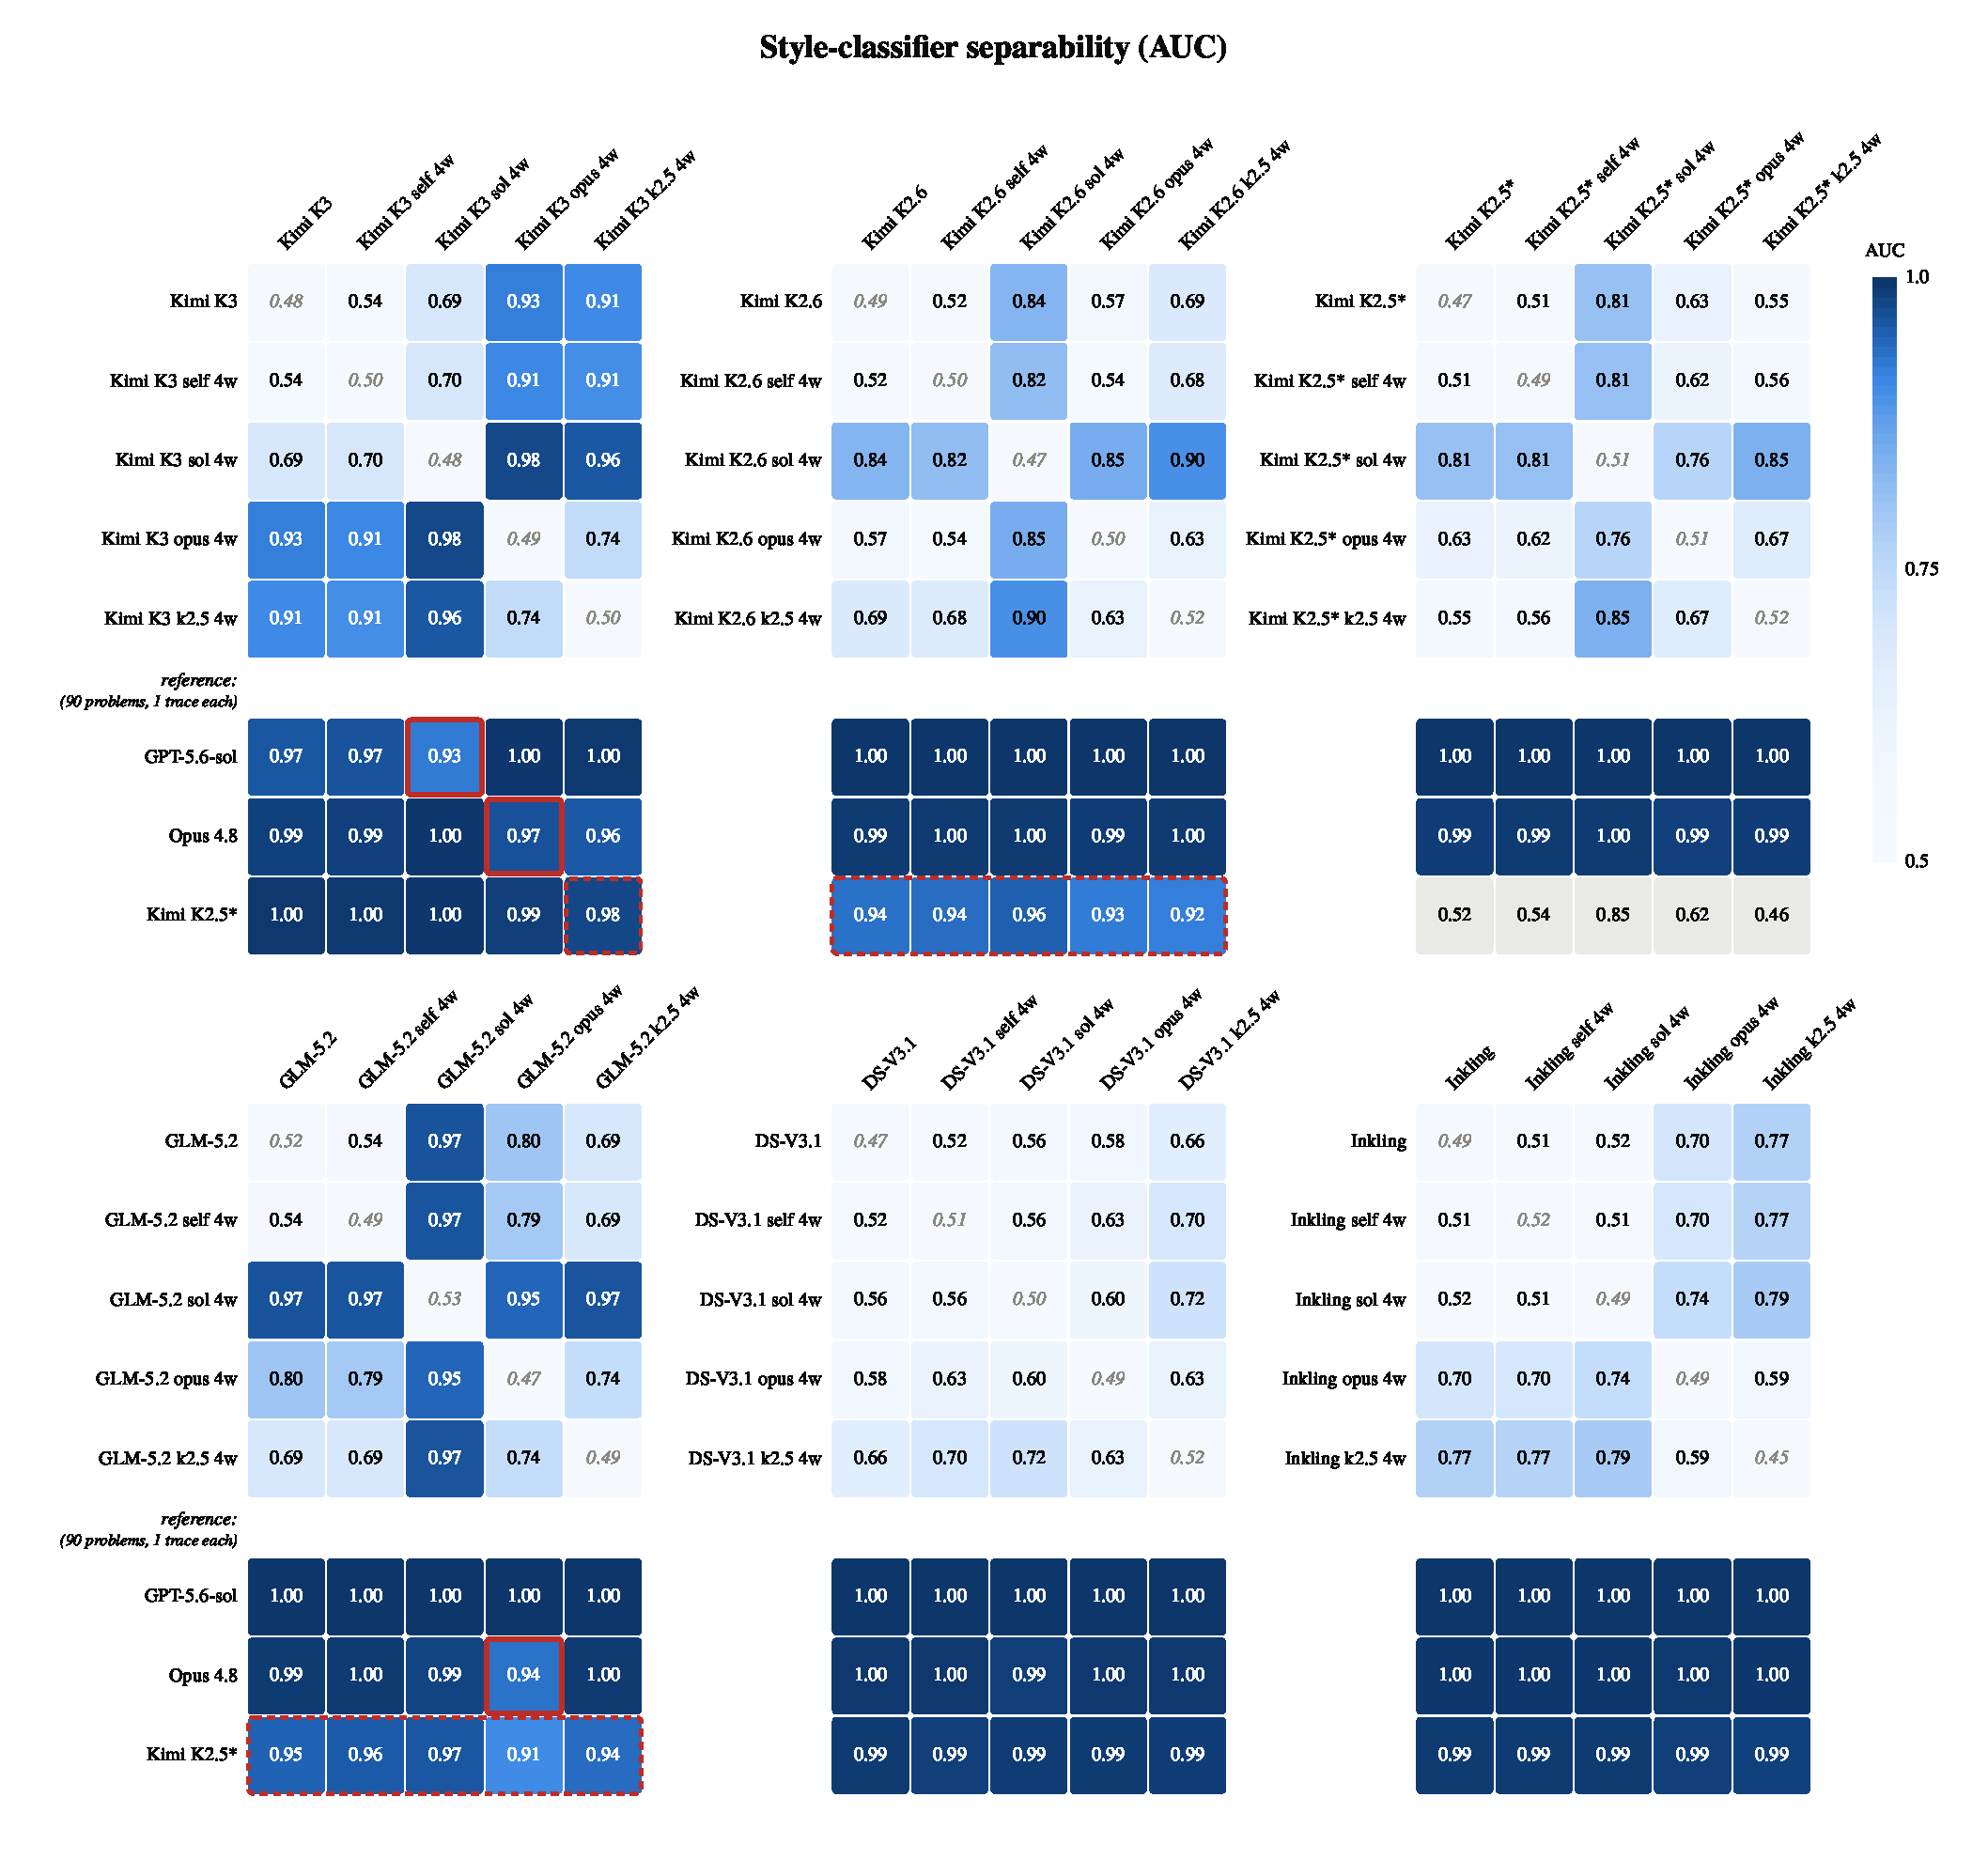
\includegraphics[trim=1cm 0 0 0, clip, width=\linewidth]{figures/thinking_prefill/len_norm_final/fig_auc_merged_4tok.pdf}
  \caption{%
Style-classifier separability with and without prefills. Each cell reports the area under the ROC curve (AUC) of a logistic-regression classifier on hashed character 3-gram to 5-gram counts, with each trace's feature vector normalized to unit length so that trace length is not available to the classifier, evaluated with five-fold cross-validation grouped by problem so that no problem appears in both training and test folds. We train a separate classifier for every cell. An AUC of 1.0 means the two trace sets are trivially distinguishable and an AUC near 0.5 means the classifier finds no generalizing stylistic boundary. Values at or below 0.6 should be read as not separable. Italic diagonal entries give each row's within-model null, obtained by splitting its own resamples. Darker blue indicates higher AUC. Each block shows one model under five conditions: no prefill, a four-word self prefill, and four-word prefills from GPT-5.6-Sol, Claude Opus 4.8, and Kimi-K2.5. Kimi-K3, Kimi-K2.6, Kimi-K2.5, and GLM-5.2 change their reasoning style under the Sol and Opus prefills (0.57 to 0.97 against their own controls), DeepSeek-V3.1 barely moves (0.56 to 0.58), and Inkling moves under the Opus but not the Sol prefill (0.70). The reference strip below each block gives the separability between the reasoning of our (prefilled) models and the reference reasoning, where a lower AUC indicates that the two are closer. Under the Sol and Opus prefills only three cells fall below their unprefilled baselines against the source the prefill was taken from, and they are outlined in red. Sol-prefilled Kimi-K3 approaches the Sol reference (0.93, from 0.97 unprefilled). Opus-prefilled GLM-5.2 and Kimi-K3 approach the Opus reference (0.94 and 0.97, from 0.99 and 0.99). The self-prefill column sits at 0.51 to 0.54 for all six models and its reference cells match the unprefilled ones to within 0.01. The Kimi-K2.5 reference row holds the 90 frozen traces that supplied the Kimi-K2.5 fragments, and its cells against Kimi-K2.5's own conditions are shaded gray because they compare the model with its own traces. the dotted red boxes mark the standing proximity of Kimi-K2.6 (0.92 to 0.96) and GLM-5.2 (0.91 to 0.97) to the Kimi-K2.5 reference, which is present without any prefill, and Kimi-K3's small movement toward the Kimi-K2.5 reference under the Kimi-K2.5 prefill (0.98, from 1.00). Note that Kimi-K2.5 is truncated at its 8,192-token serving cap in all rows due to prefill-API limitations.%
}
  \label{fig:auc-prefill-and-control}
\end{figure}

\begin{figure}[H]
  \centering
  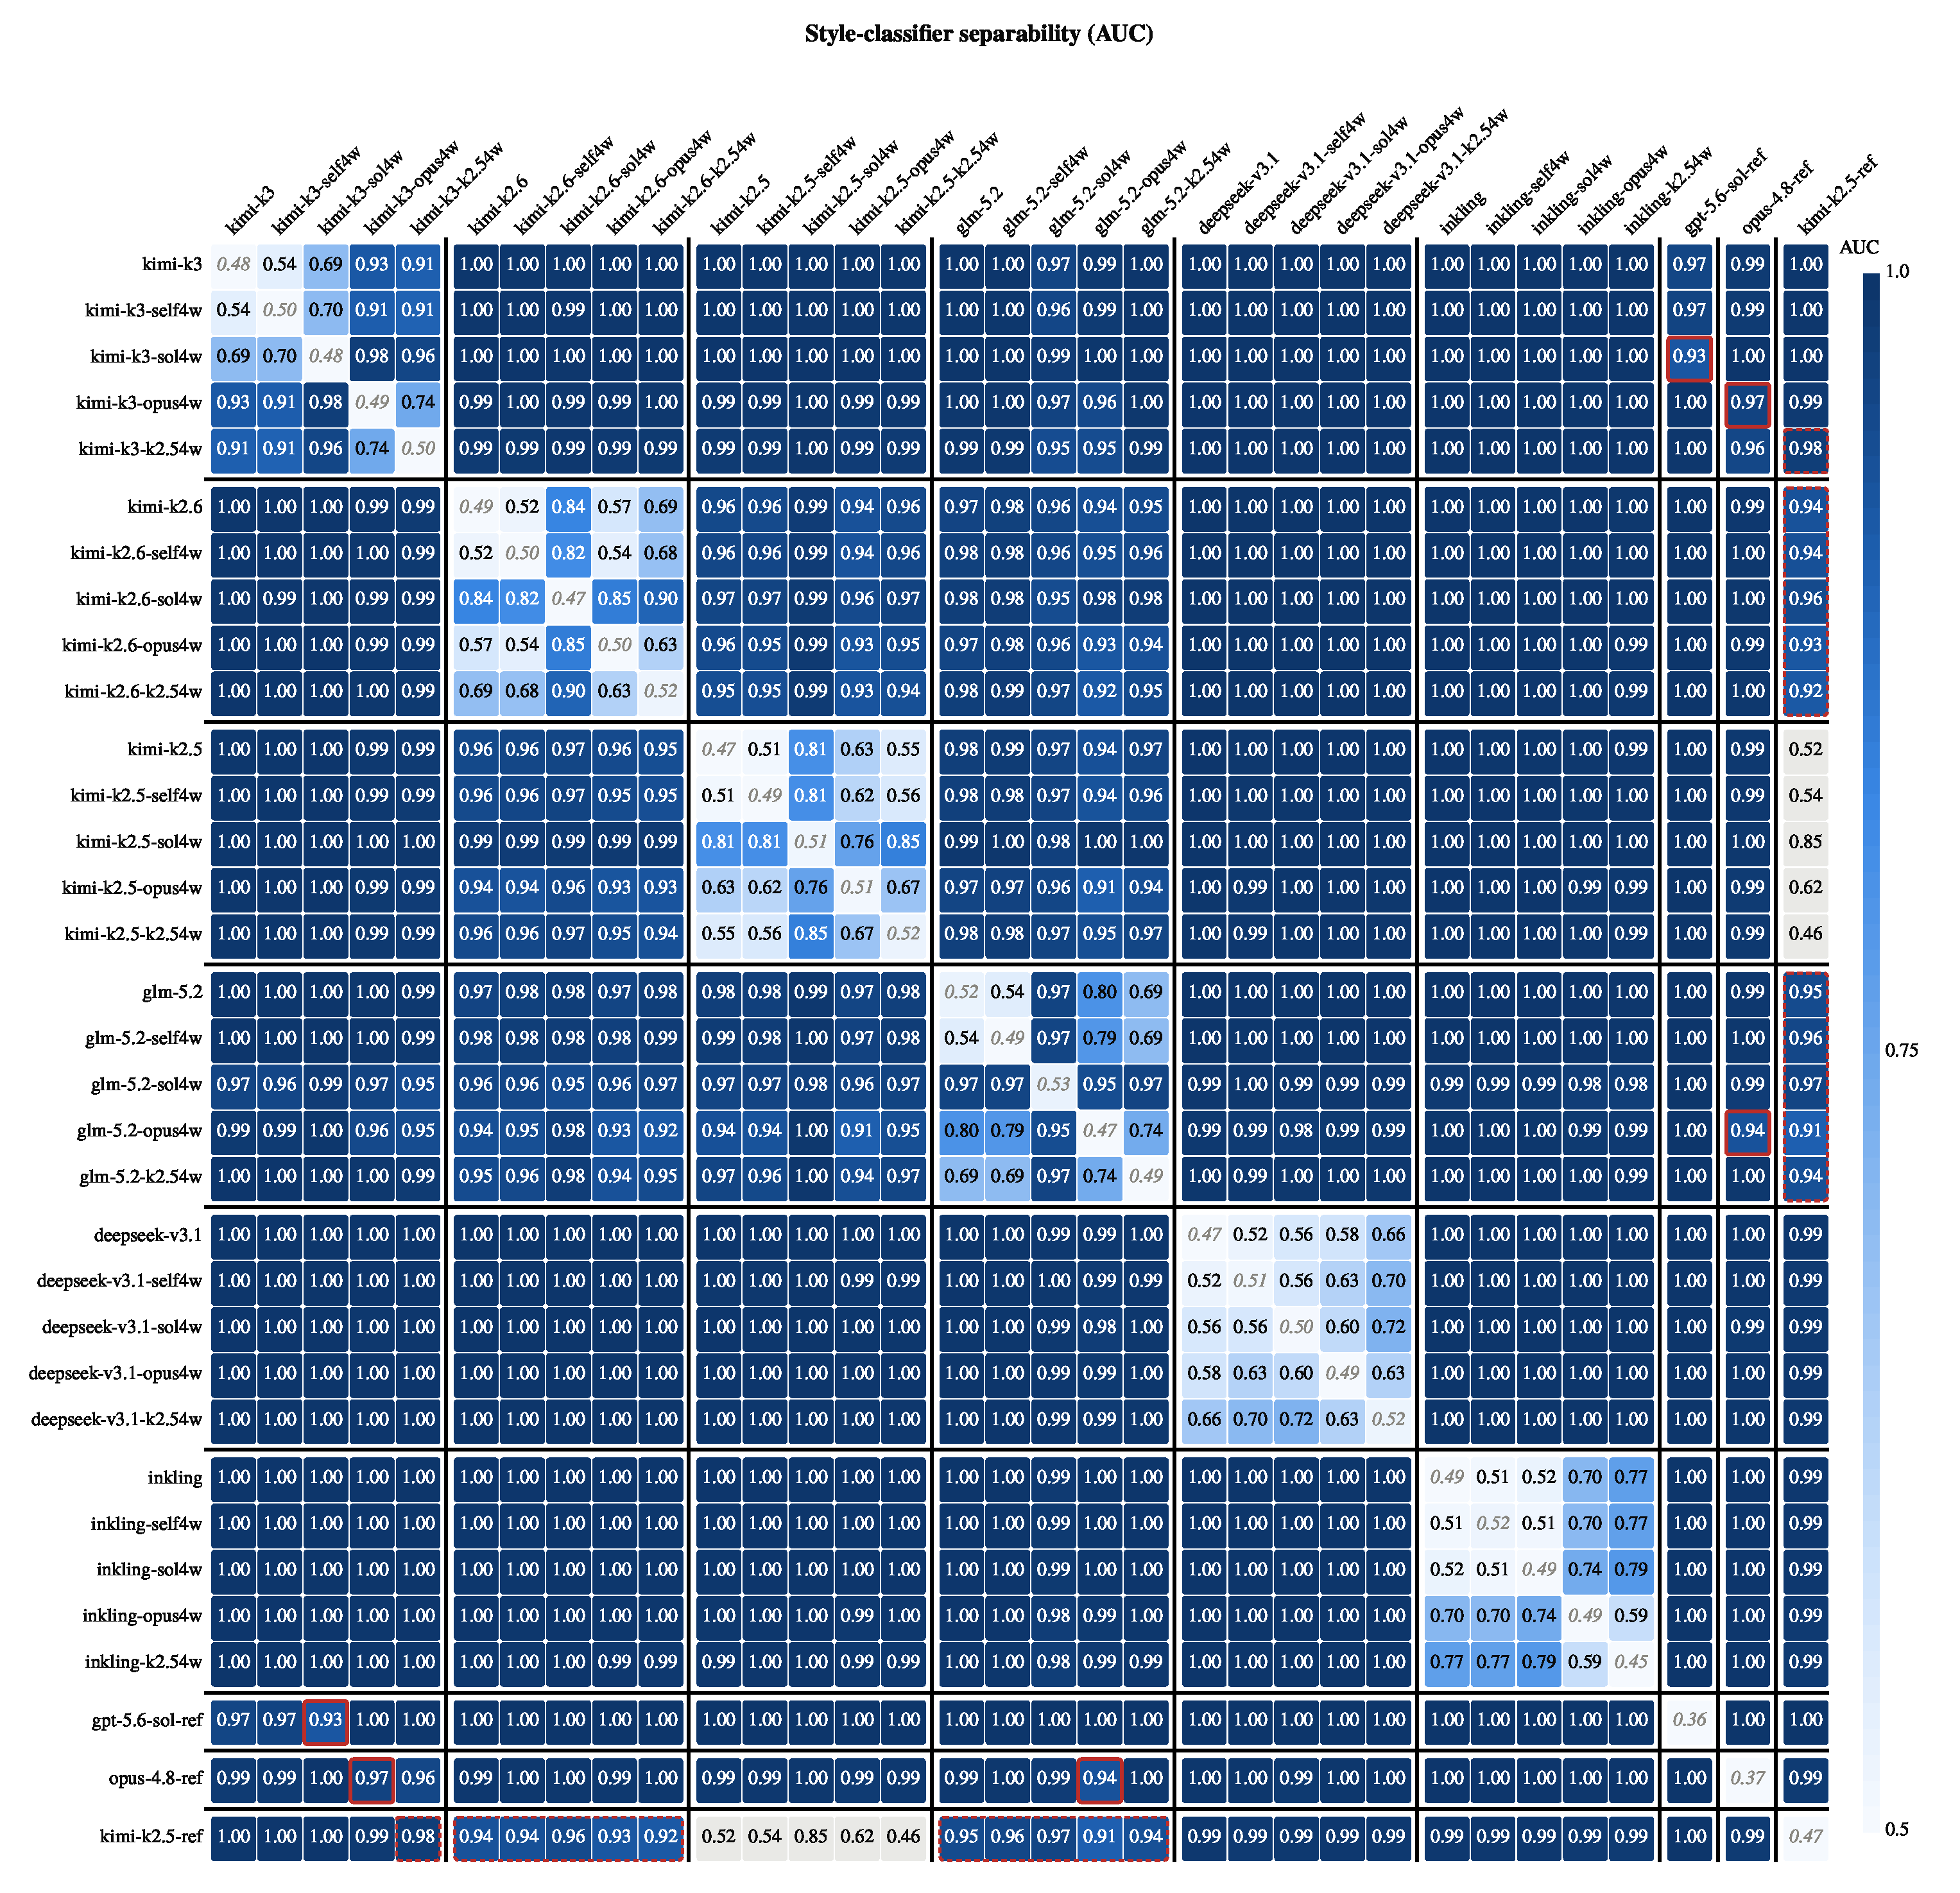
\includegraphics[width=\linewidth]{figures/thinking_prefill/len_norm_final/fig_auc_matrix_4tok.pdf}
  \caption{Full 33-row classifier matrix over all models, conditions, and references, same classifier and color scale as \Cref{fig:auc-prefill-and-control}. Black rules separate models and the reference block. Italic diagonal entries are within-model nulls. The reference rows hold one trace per problem, so their nulls (0.36 to 0.47, bottom right) sit below 0.5 as described in \Cref{app:drift_setup}, and their cells are not comparable with the 360-versus-360 cells at face value. The three cells where the prefill moves models closer to the source model of the prefill are outlined in red in both their row and column positions. Cells comparing Kimi-K2.5 with its own teacher reference are shaded gray, and the dotted red boxes mark the standing proximity of Kimi-K2.6 and GLM-5.2 to the Kimi-K2.5 reference.}
  \label{fig:auc-prefill-full}
\end{figure}

\subsubsection{Distinctive $n$-gram Overlap}\label{app:drift_phrases}

\paragraph{Method.}
We score word $n$-grams with $n \in \{1, 2, 3\}$. Reasoning is lowercased and tokenized to alphabetic word runs, so numbers and operators drop out. Each row of the matrix is one model under one condition, or one reference, with all of its traces pooled. Every n-gram with at least ten pooled occurrences is scored by the log-odds z-score of the row against a fixed background, with an informative Dirichlet prior following \citet{monroe2008fightin}. The background is the pool of the six unprefilled open-weight model rows. It contains no prefill conditions and no references, so vocabulary common to the models on these problems cancels. Furthermore, an $n$-gram that several models adopt from a source remains distinctive of each of them. The forty highest-scoring n-grams form a row's characteristic list, and a cell reports the Jaccard overlap of two such lists. Because both lists hold forty $n$-grams, the union shrinks as the overlap grows.

\paragraph{Results.}
The results are similar to the classifier results. The three cells outlined in red, Sol-prefilled Kimi-K3 against the Sol reference and Opus-prefilled Kimi-K3 and GLM-5.2 against the Opus reference, carry the most substantial $n$-gram overlaps (\Cref{fig:ngram-prefill-and-control}). Kimi-K3 shares 12 $n$-grams of a union of 68 with the Sol reference already without any prefill (0.18), rising to 13 of 67 under the Sol prefill (0.19); this standing Sol overlap persists under the self prefill (0.16) and is displaced by the Opus and Kimi-K2.5 prefills (0.00 and 0.03). The Opus overlaps are largest under the Opus prefill. Opus-prefilled Kimi-K3 shares 12 of 68 with the Opus reference (0.18) and Opus-prefilled GLM-5.2 shares 15 of 65 (0.23). Without the prefill, both overlaps are zero. A reduced version of the same overlap appears under the Kimi-K2.5 prefill (0.13 for Kimi-K3 and 0.08 for GLM-5.2), matching the partial classifier movement noted in \Cref{app:drift_classifier}. The shared $n$-grams are a small number of recurring mannerisms rather than broad vocabulary: hedged assessment terms such as \textit{perhaps}, \textit{likely}, \textit{could}, and \textit{exact} for the Sol pair, and variations of \textit{hmm let me reconsider} and \textit{let me think about} for the Opus pairs. Overlapping n-gram lengths mean one habit contributes several list entries, so the overlap reads as shared signature mannerisms rather than a count of independent behaviors. 
%Within the family, Kimi-K2.5 overlaps its own teacher traces at 0.21 unprefilled, while the Sol and Opus prefills displace even this self-overlap to 0.03 and 0.11. 
Kimi-K2.6 picks up 9 $n$-grams of the teacher's list under the Kimi-K2.5 prefill (0.13, against 0.00 to 0.01 under the control, self, and Sol conditions).
The Opus prefill also lifts it to 0.11, through shared mathematical notation such as \textit{bmod} and \textit{setminus} rather than shared mannerisms.
Surprisingly, under a prefill of the same four-word length, Kimi-K2.6 thus picks up fewer of Kimi-K2.5's characteristic $n$-grams (0.13) than Kimi-K3 and GLM-5.2 pick up of Opus 4.8's (0.18 and 0.23), and fewer than Kimi-K3 shares with the Sol reference (0.19), most of which exists without any prefill.
% Surprisingly, under a prefill of the same four-word length, Kimi-K2.6 thus picks up fewer of Kimi-K2.5's characteristic $n$-grams (0.13) than GLM-5.2 picks up of Opus 4.8's (0.23).

\begin{figure}[H]
  \centering
  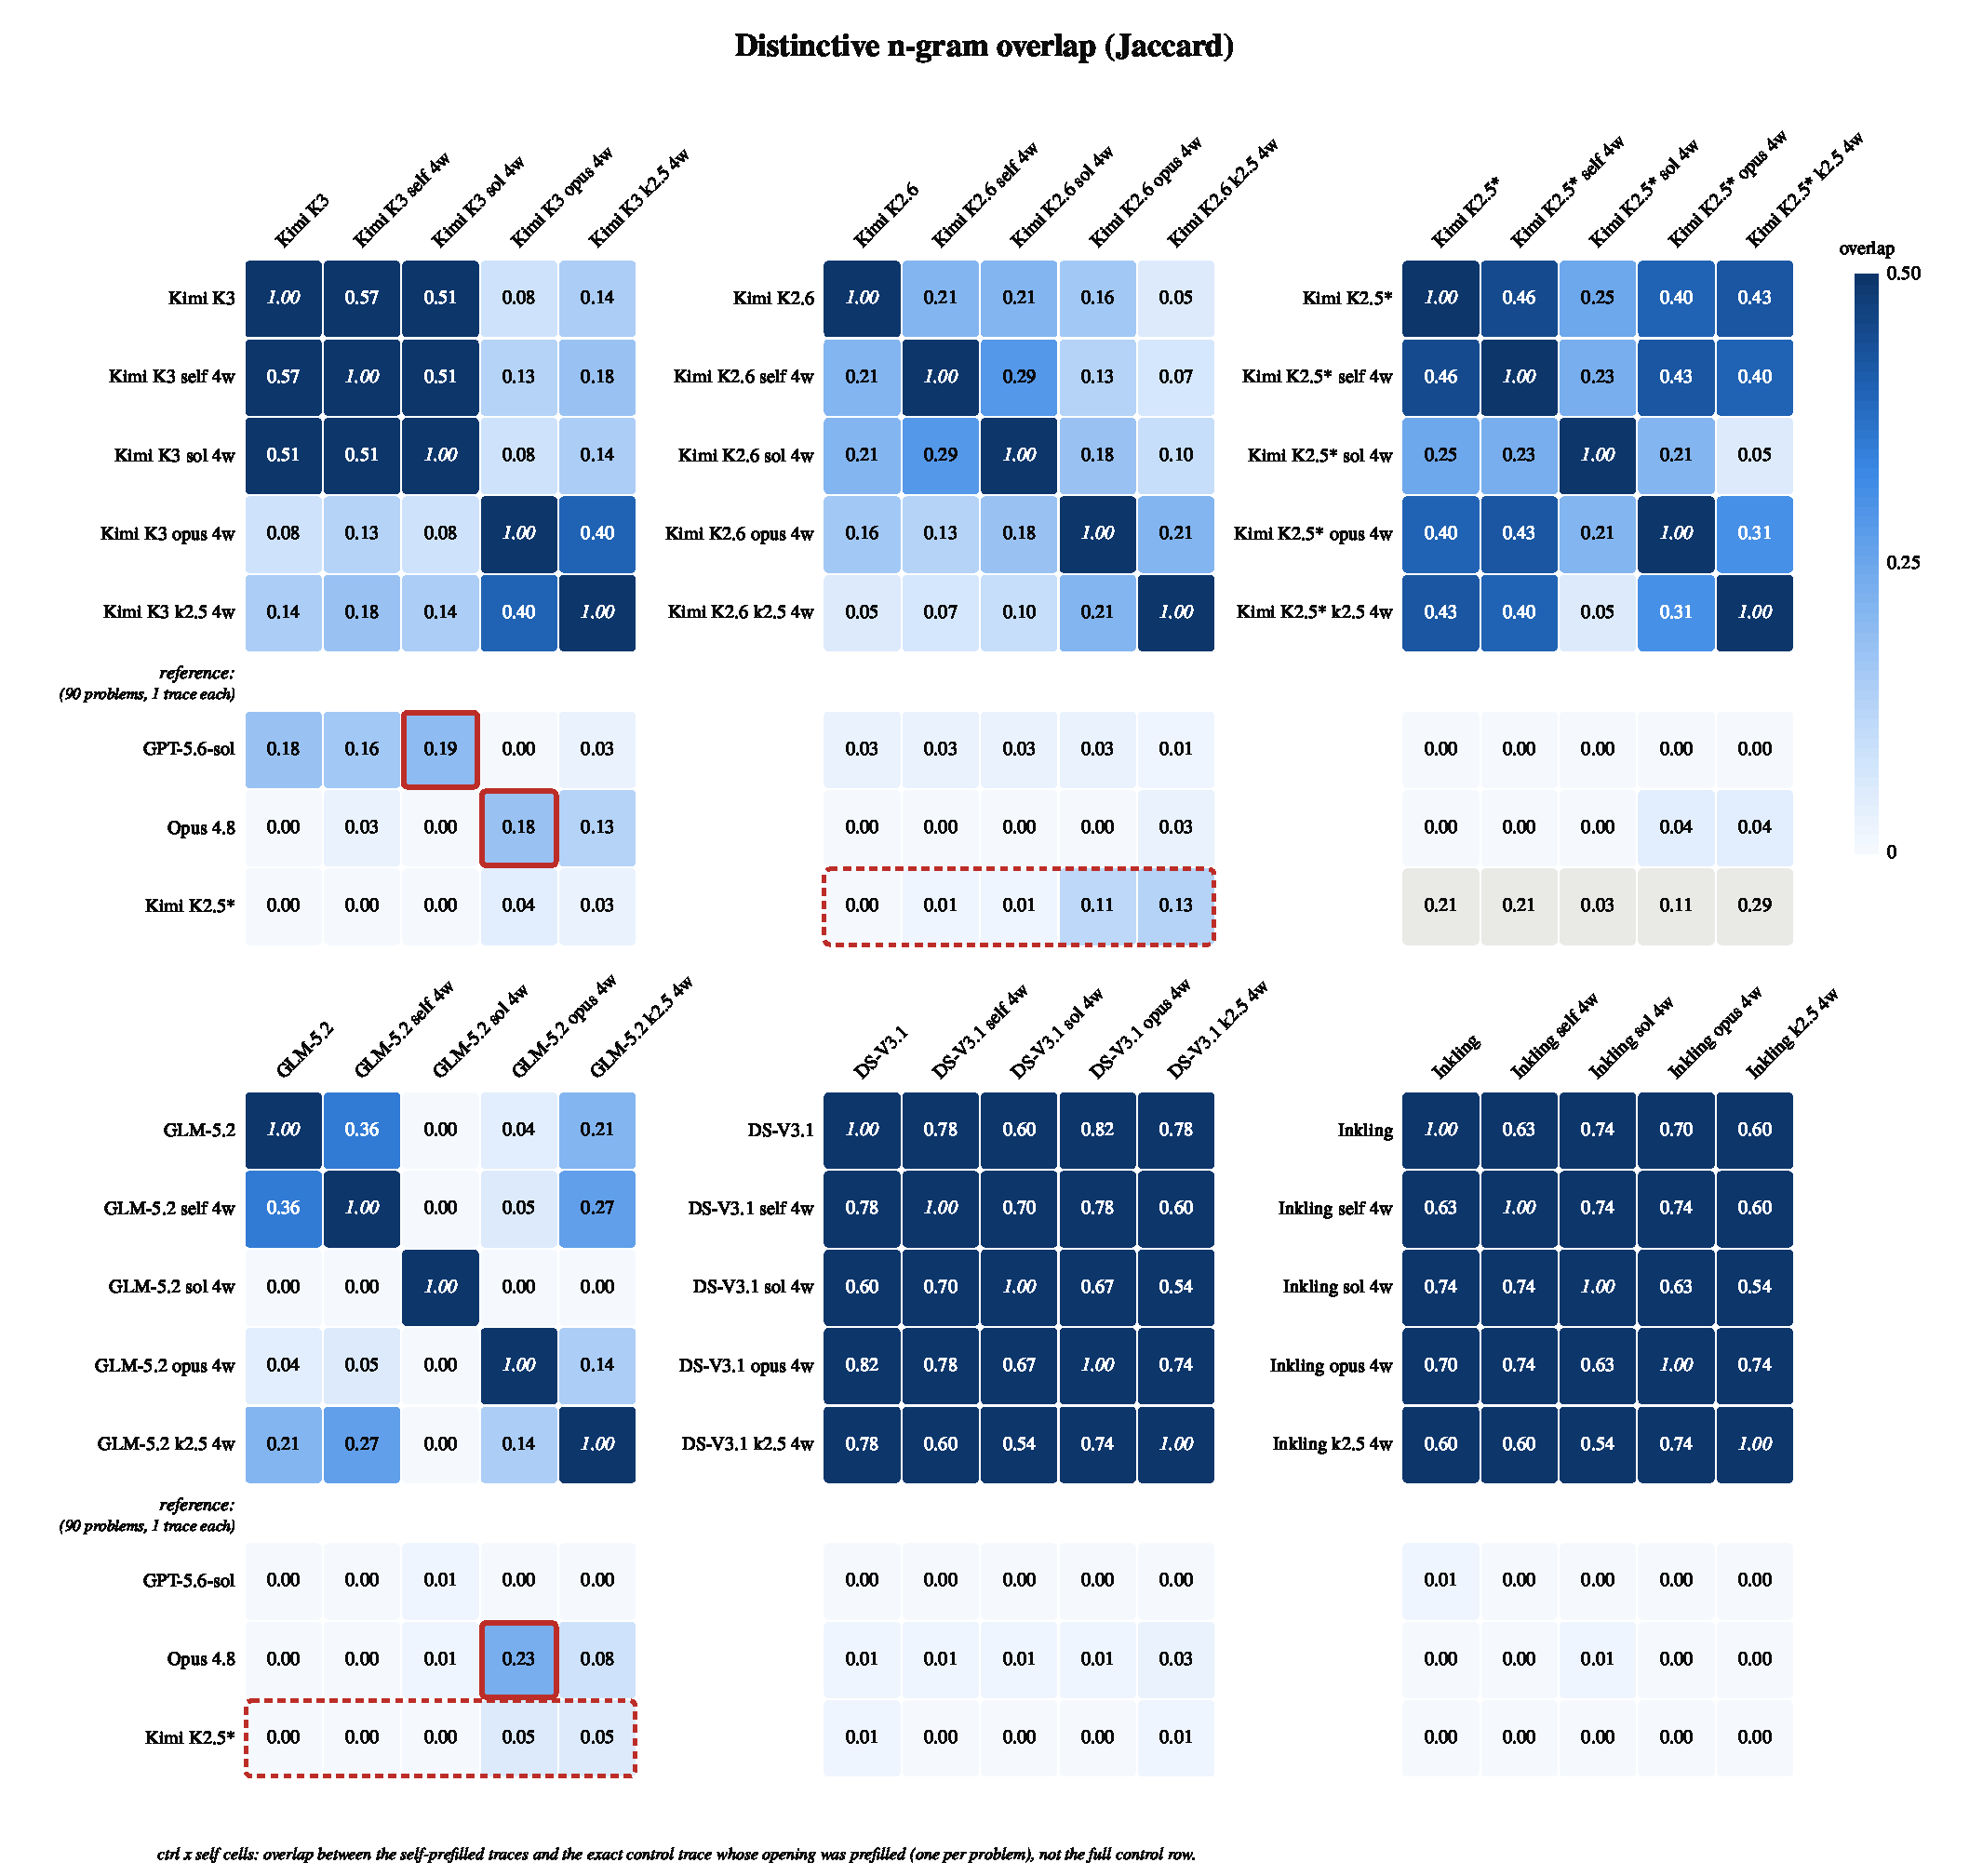
\includegraphics[trim=1cm 1cm 0 0, clip, width=\linewidth]{figures/thinking_prefill/len_norm_final/fig_ngram_merged_4tok.pdf}
  \caption{%
  Distinctive n-gram overlap under prefills. Each cell reports the Jaccard overlap of the two rows' most characteristic $n$-grams, scored against the pooled unprefilled controls as described in \Cref{app:drift_phrases}. Darker hue indicates more shared $n$-grams and the diagonals are one by definition. The square blocks show the same five conditions as \Cref{fig:auc-prefill-and-control}. The reference cells are near or at zero everywhere except the Kimi-K3 vs Sol cells, the three cells outlined in red, and a few Kimi-K2.5-prefill cells. Sol-prefilled Kimi-K3 shares characteristic $n$-grams with the Sol reference (0.19, from 0.18 without any prefill). Opus-prefilled Kimi-K3 and GLM-5.2 share $n$-grams with the Opus 4.8 reference (0.18 and 0.23). The control-versus-self cells compare the self-prefilled traces against the exact control trace whose opening was prefilled, one per problem. The reference cells of the self column match the unprefilled ones to within 0.03. In the Kimi-K2.5 reference row, the gray cells compare Kimi-K2.5 with its own teacher traces, and Kimi-K2.6 shows a small overlap with the teacher chiefly under the Kimi-K2.5 prefill (0.13, dotted red row) and to a lesser degree under the Opus prefill (0.11).
  Note that Kimi-K2.5 is truncated at its 8,192-token serving cap in all rows due to prefill-API limitations.%
  }
  \label{fig:ngram-prefill-and-control}
\end{figure}

\subsubsection{Response to Prefill Length}\label{app:drift_dose}

To study the sensitivity to prefill length, we vary the prefill length from 0 to 16 words for the Sol and Opus sources, holding everything else fixed. A cue should take effect within a few words and then flatten, whereas a model learning from the fragment should keep changing as it receives more.

All three movements, Kimi-K3 toward either reference and GLM-5.2 toward the Opus reference, behave more like cues. Against the Opus reference, GLM-5.2 drops to AUC 0.96 at a single word, flattens after eight, and ends at 0.92 at 16 words, while Kimi-K3 drops to 0.97 at a single word and stays between 0.95 and 0.97 at every length (\Cref{fig:dose-auc}). Against the Sol reference, Kimi-K3 descends from 0.96 unprefilled to 0.93 at 4 words and saturates more slowly, reaching 0.89 at 16 words. Phrase overlap follows the same pattern (\Cref{fig:dose-ngram}): GLM-5.2 acquires Opus phrasing at a single word (0.23), and Kimi-K3's Opus overlap completes near four words (0.18), while its Sol overlap is present without any prefill and grows under Sol prefills to 0.27 at 16 words. DeepSeek-V3.1, Inkling, Kimi-K2.6, and Kimi-K2.5 remain at or above AUC 0.98 and at most 0.05 phrase overlap against both sources at every length tested.
GLM-5.2 shows no classifier drift toward the Sol reference (0.999 to 1.00 at every length), but its Sol phrase overlap grows slowly from zero to 0.04 at 12 to 16 words, far below Kimi-K3 against either reference and GLM-5.2 against the Opus reference.
Note that these trends are noisy as every point rests on a limited data set of the same 90 problems.

\begin{figure}[H]
  \centering
  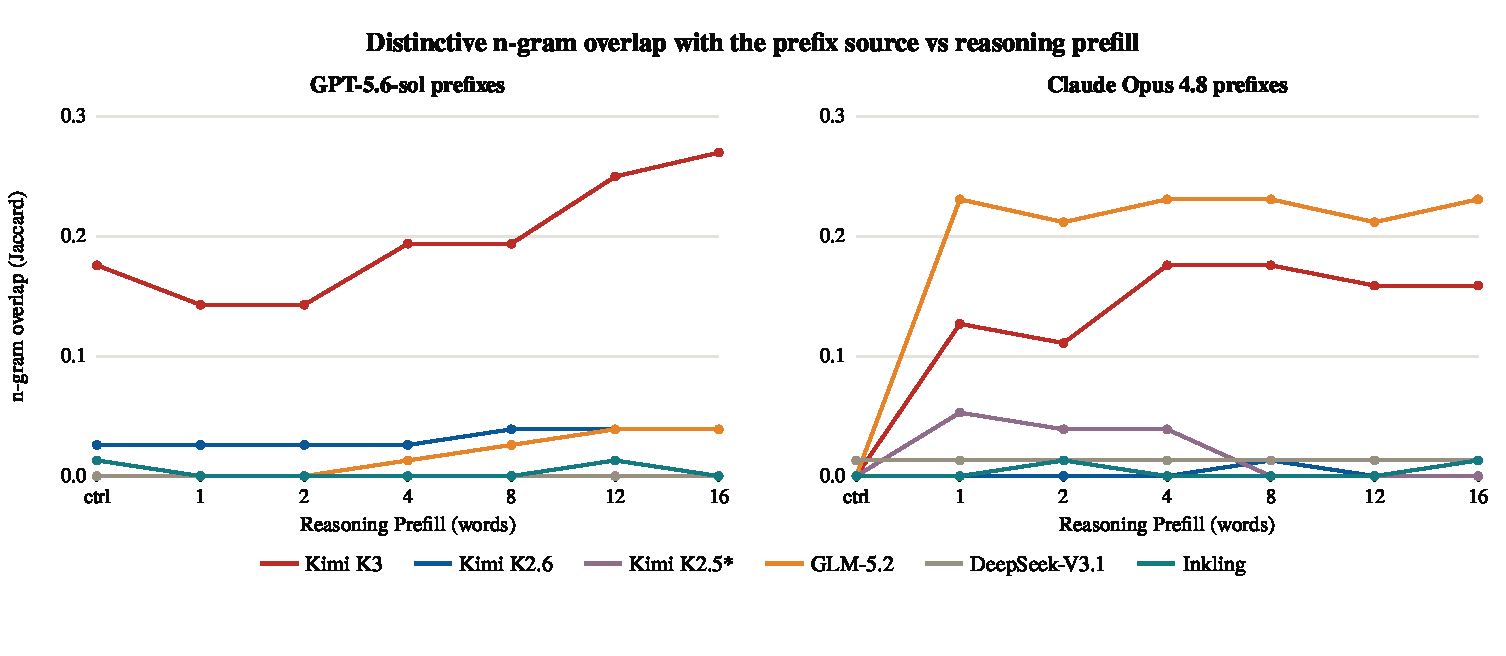
\includegraphics[width=\linewidth]{figures/thinking_prefill/len_norm_final/fig_dose_ngram.pdf}
  \caption{%
    Overlap of characteristic phrases with the prefill source as a
    function of prefill length in words. Each point is the Jaccard overlap between a
    model's most distinctive n-grams and those of the decoded reference,
    with the unprefilled control as the leftmost point. DeepSeek-V3.1,
    Inkling, Kimi-K2.6, and Kimi-K2.5 are at or near zero overlap with both sources at
    every length. Kimi-K3 shares Sol phrasing already without any prefill
    and gains further under Sol prefills, to 0.27 at 16 words. GLM-5.2 acquires Opus phrasing
    at a single word and Kimi-K3 follows once its
    Opus register change completes around 4 words. GLM-5.2's overlap with the Sol reference grows slowly and peaks at 0.04 at 12 to 16 words.
  }
  \label{fig:dose-ngram}
\end{figure}

\begin{figure}[H]
  \centering
  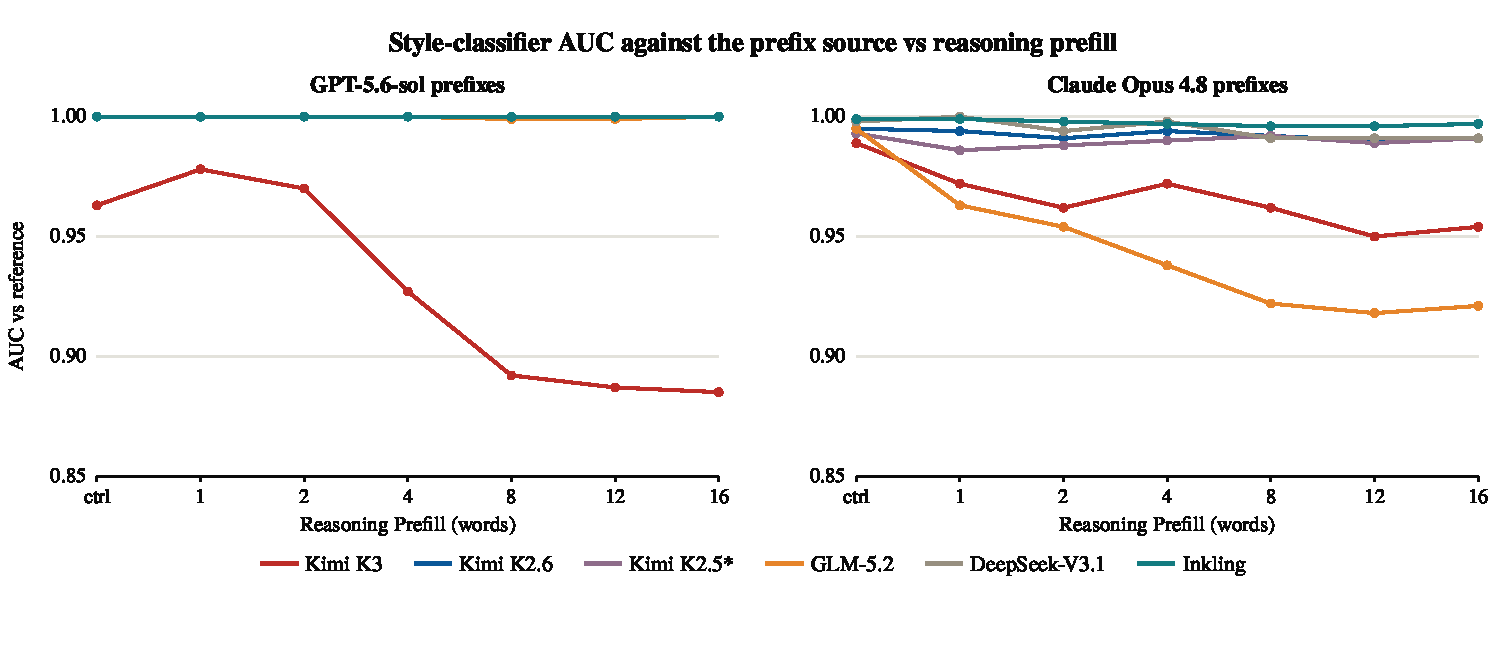
\includegraphics[width=\linewidth]{figures/thinking_prefill/len_norm_final/fig_dose_auc.pdf}
  \caption{%
    Style-classifier separability from the prefill source as a function
    of prefill length in words. Lower means the prefilled reasoning is harder to
    tell apart from the decoded reference. The axis is cut at 0.85. The adoption floor measured on the self-prefill calibration, where the reference is the model's own trace, lies below the
    plotted range. DeepSeek-V3.1, Inkling, Kimi-K2.5, and Kimi-K2.6 sit at or above 0.98 against both references at every length.
    Kimi-K3 descends against the Sol reference from 0.96
    unprefilled to 0.89 at 16 words. GLM-5.2 descends
    against the Opus reference to 0.92 at 16 words, while Kimi-K3 stays between 0.95 and 0.97 against Opus. GLM-5.2 shows no drift toward the Sol reference (0.999 to 1.00 at every length).%
  }
  \label{fig:dose-auc}
\end{figure}

\subsubsection{Reasoning-Length Distributions}\label{app:drift_length}

The next property we examine is reasoning length. We count each trace in tokens with the Kimi-K3 tokenizer and compare per-model length distributions across conditions. Length complements the preceding analyses because it captures how long a model deliberates rather than how it writes, and because the classifier's normalized features exclude it. A four-word prefill contains no statement of a reasoning budget, so a length response cannot be copied from the prefill. It has to come from the model.

In general, the reference traces are far shorter than the reasoning of the tested open-weight models. The median reference lengths are 1{,}700 tokens for GPT-5.6-Sol and 1{,}100 for Opus 4.8, against unprefilled medians of 5{,}700 to 25{,}400 for the six models.

\Cref{fig:length-distributions-4tokens} shows the distributions. DeepSeek-V3.1, Inkling, and Kimi-K2.6 keep their unprefilled lengths under every prefill. Kimi-K3 and GLM-5.2 shorten. Under the Opus prefill, Kimi-K3's median falls from 5{,}700 to 2{,}500 tokens, roughly twice the source median, and GLM-5.2's falls from 17{,}600 to 7{,}800. Under the Sol prefill the shortening is weaker, to 4{,}400 and 12{,}200. Under the Kimi-K2.5 prefill the same two models shorten as well, to 3{,}500 and 10{,}100, so part of the shortening is generic.

In the self condition, five models keep their unprefilled lengths. Kimi-K3 shortens mildly, to a median of 5{,}100 against 5{,}700, the largest self-condition length change we observe. Its Sol and Opus shortenings (4{,}400 and 2{,}500) clearly exceed this. Under the Opus prefill, Kimi-K3's per-problem lengths also correlate somewhat more strongly with the per-problem source lengths, at a Spearman correlation of 0.86 against 0.77 without the prefill.

\begin{figure}[H]
  \centering
  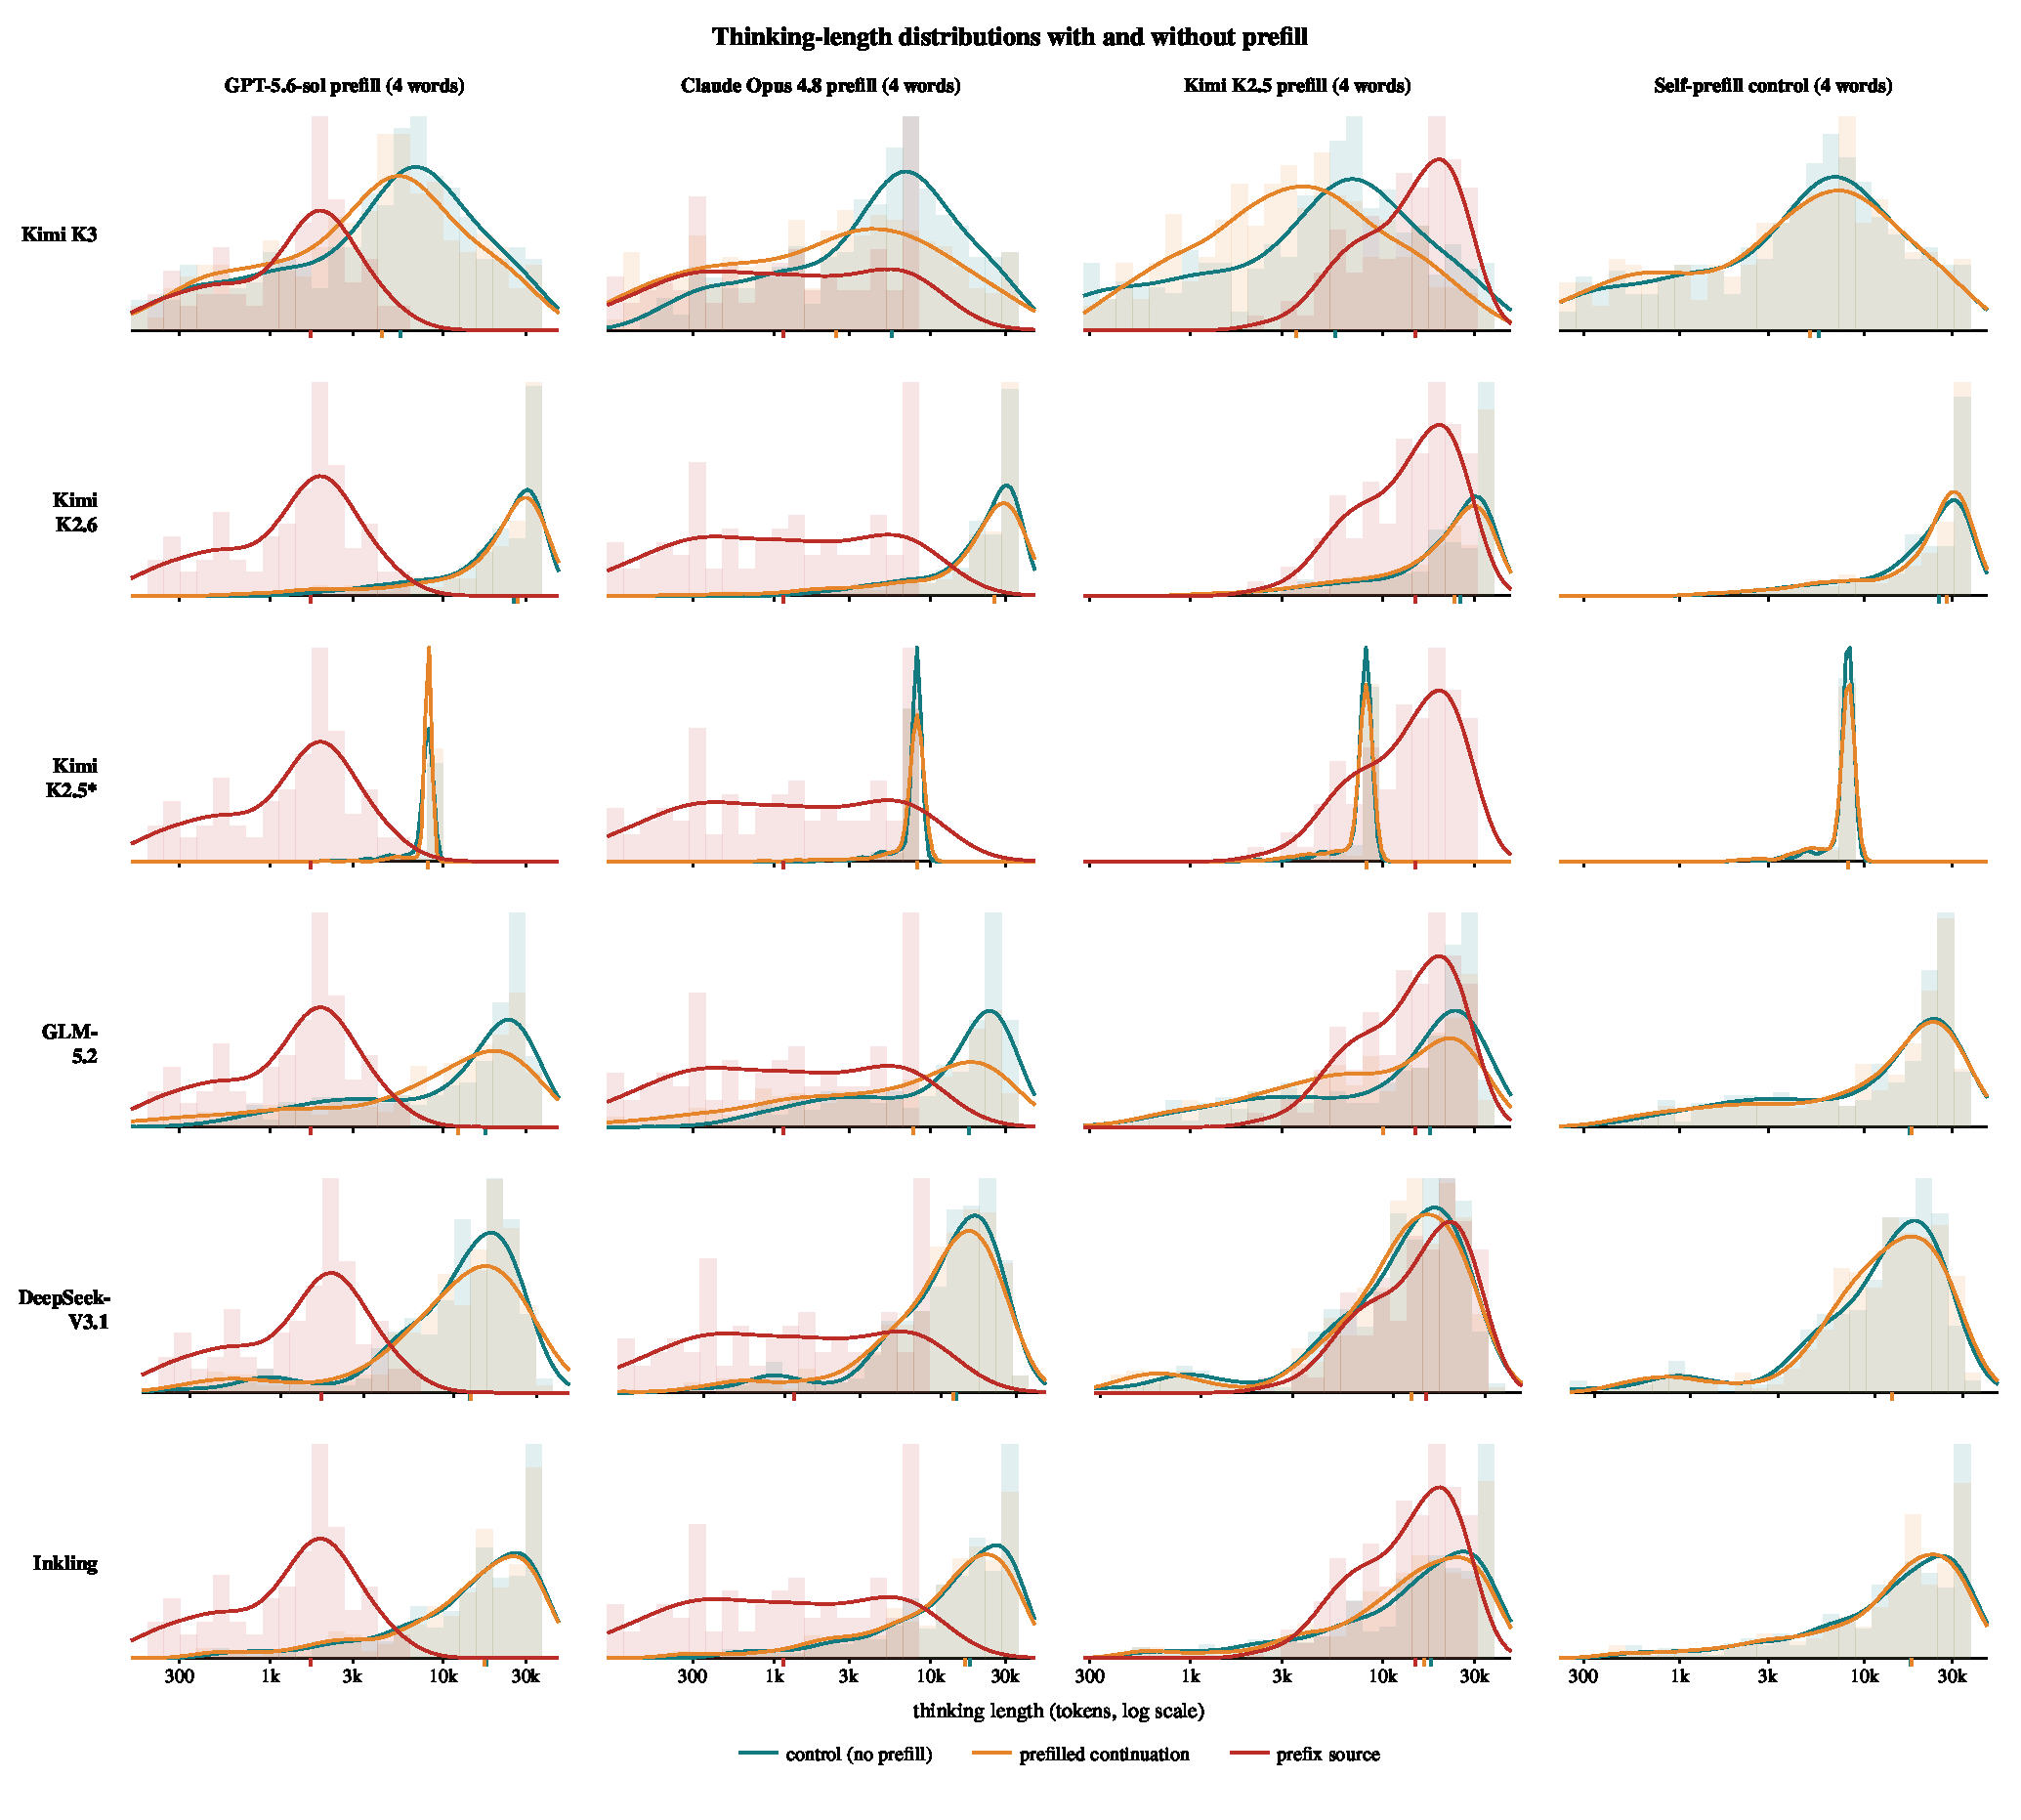
\includegraphics[trim=0 0 0 1cm, clip, width=\linewidth]{figures/thinking_prefill/len_norm_final/fig_length_distributions_4tok.pdf}
\caption{%
    \textbf{Reasoning-length distributions with and without prefills.} Each panel shows kernel density estimates of per-trace reasoning length in tokens on a logarithmic axis. Teal shows the model's control reasoning length without prefill. Orange shows the same model's continuations after the prefill. Red shows the reasoning length of the source traces that supplied the prefill. Small ticks below each axis mark the median of the matching distribution. Rows correspond to models. The columns use prefills from GPT-5.6-Sol, Claude Opus 4.8, Kimi-K2.5, and, as a control, a reasoning prefill from a previous rollout of the same model. All available resamples enter the densities, roughly 360 traces per model-condition and 90 per source. GPT-5.6-Sol and Opus 4.8 think far more briefly than any open model.
    The Kimi-K2.5 row looks different for a mechanical reason. Its own traces are cut at the 8{,}192-token serving cap and pile up there, while the red teacher traces were collected without the cap, so the row shows the cap rather than the model's reasoning budget.
    For DeepSeek-V3.1, Inkling, and Kimi-K2.6 the orange curve is close to the unprefilled distribution (teal) in every panel, so the prefill leaves their reasoning budget untouched. However, Kimi-K3 and GLM-5.2 shift toward shorter reasoning under foreign prefills, most strongly under Opus. %In the self column the orange curve lies on the teal for five models and Kimi-K3 shows a mild shortening (median 5{,}100 against 5{,}700).
  }
  \label{fig:length-distributions-4tokens}
\end{figure}


